\section{Decision objectives and success-grader sensitivity}
\label{app:ablations}
The protocol was frozen before execution of this additional study, after
the original simulation study had been inspected. All ten cases use 500
independent repetitions, 6,000 pairs, master seed 2026091804, and looks
at 100 and every 100 pairs thereafter. The same 40 positive bets and
same-look conjunction are used. Fixed weighted utility is
$0.8S+0.1C+0.1/(1+\mathrm{cost})$; bounded efficiency is
$1/(1+\mathrm{cost})$. Both are in $[0,1]$, so their pair differences
use the same bounded-score betting construction. Their cost scale and
weights are illustrative preferences, fixed before seeing this study.
Giving utility to cost on unsuccessful episodes differs from the
hierarchical resource-eligibility rule.

The six compared decisions require respectively: success superiority;
only success/compliance noninferiority; guarded hierarchical preference;
utility superiority; guarded utility superiority; or guarded efficiency.
An approval is not labeled a statistical error solely because another
method's different deployment region fails. Population Pareto labels use
true success, compliance and raw mean cost; they are descriptive facts of
the generating laws, not estimated confidence regions. Mean lognormal
cost is analytic, and bounded-efficiency means use Gauss--Hermite
quadrature with 80/160-node agreement checked.

\paragraph{What can a known label-error guarantee protect?}
For an iid episode-pair law let $\widetilde S$ be a measured success bit
and suppose $P(\widetilde S^a\ne S^a)\leq\epsilon_a$ for $a=A,B$.
All other metrics and the frozen comparison rule agree. Put
$\epsilon=\epsilon_A+\epsilon_B$. A union bound and bounded scores give
\[
 |\widetilde\Delta_S-\Delta_S|\leq\epsilon,\qquad
 |\widetilde\theta-\theta|\leq2\epsilon.
\]
Indeed a success difference can change by at most the sum of its two
label-error indicators, and the hierarchical sign changes by at most
two on the event that at least one label is wrong. Taking expectations
proves both bounds. Hence measured superiority thresholds
$2\epsilon$ for net benefit and $-0.03+\epsilon$ for success,
with unchanged compliance threshold, suffice for the true deployment
region. For the iid study, the corresponding fixed conditional nulls
and intersection--union proof give the same anytime false-deployment
bound. Under temporal adaptation, analogous conditional error bounds
would need independent justification. Uncertainty in estimated grader
error rates is not covered by treating those estimates as known constants.

The four noise cases use conditional false-positive/false-negative rates
(FP,FN): identical agents with (.05,.05) in both arms; a true success
harm (.71 versus .75) with $A=(.05,0)$ and $B=(0,.05)$; an efficiency
gain (.75 versus .75, cost ratio .55) with the adverse reverse pattern;
and larger true harm (.65 versus .75) with (.05,.05) in both arms.
For the harm cases the cost ratio is .4. All compliance probabilities
are .995. Noise is independent of cost and compliance conditional on
true success and arm. The measured success probability is
$p(1-\mathrm{FN})+(1-p)\mathrm{FP}$, which gives the analytic measured
hierarchical target after substitution in the original target formula.
The conservative armwise error bound is $\max(\mathrm{FP},\mathrm{FN})$;
it may exceed the actual unconditional error frequency.

For favorable differential grading of the smaller harm,
the 97.8\% measured approval rate has Wilson 95\% Monte Carlo interval
$[96.10\%,98.77\%]$. True-label and conservative-bound approvals are
zero in 500 repetitions. With adverse differential labels on a real
efficiency gain, true-label approval is 73.8\% and measured approval is
zero. These results concern the four stated noise laws. They do not
validate a real judge, recover latent truth without assumptions, or
establish power of the conservative correction. In all four cases, the
assumed summed error bound is 0.10, making its measured-success threshold
$0.07$; every measured contrast is below that threshold. Thus all four
are null cases for this sufficient rule, and no bound-aware alternative
was studied. Zero approvals are not evidence of corrective power.

\begin{figure}[h]
\centering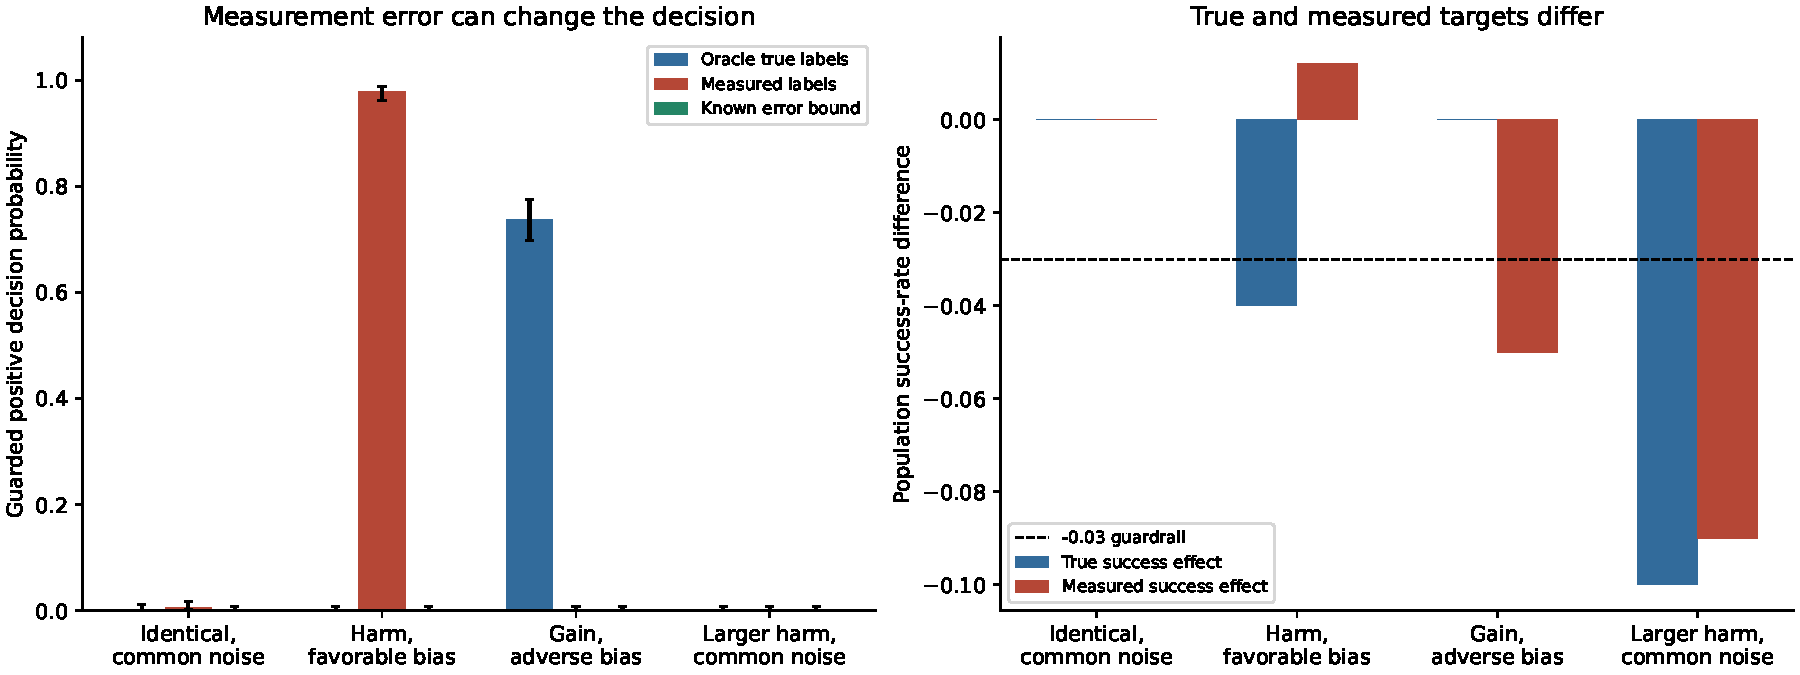
\includegraphics[width=\linewidth]{../results/decision_ablation_grading.pdf}
\caption{Success-grader sensitivity under four fixed noise laws. Oracle
labels exist only in simulation; the bound-aware rule assumes externally
valid error limits. Rates are Monte Carlo decisions about the indicated
measured or true target, not evidence about an actual deployed grader.}
\end{figure}
